\documentclass[tikz]{standalone}

\usepackage{xcolor}
\definecolor{stgoblue}{RGB}{74,144,226}
\definecolor{stgogreen}{RGB}{80,227,194}
\definecolor{stgored}{RGB}{255,69,0}
\definecolor{stgoorange}{RGB}{255,165,0}

\usetikzlibrary{fit,shapes.geometric}

\begin{document}

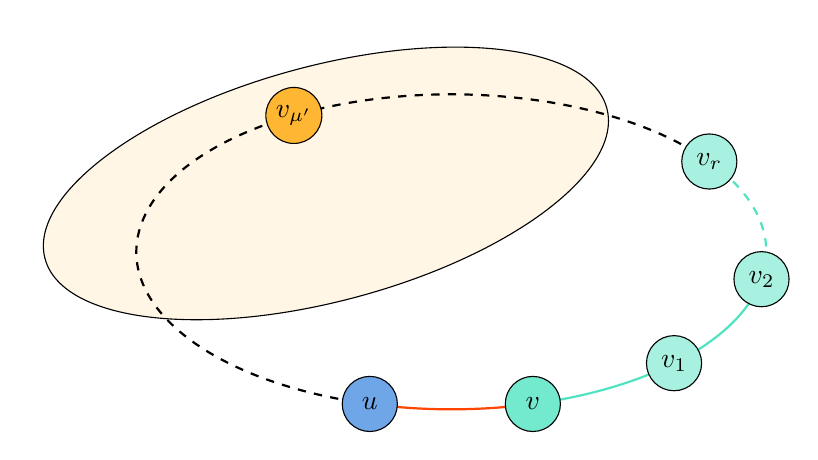
\begin{tikzpicture}
    % Node styles
    \tikzstyle{nodeStyle}=[circle, draw, fill=white, inner sep=2pt, 
      minimum size=7mm]

    % Define ellipse parameters
    \def\radiusA{4cm}
    \def\radiusB{2cm}
    \def\radius{{\radiusA} and \radiusB}

    % Define positions
    \coordinate (u) at (255:\radius);
    \coordinate (v) at (285:\radius);
    \coordinate (v1) at (315:\radius);
    \coordinate (v2) at (350:\radius);
    \coordinate (vr) at (35:\radius);
    \coordinate (w) at (120:\radius);

    % Draw neighborhoods
    \node[draw,fill=stgoorange!10,ellipse,
      rotate fit=15,fit=(w) (200:\radius) (80:\radius)] {};

    % Draw edges
    \draw[thick,stgored] (u) 
      arc[start angle=255, end angle=285, x radius=\radiusA, y radius=\radiusB];
    \draw[thick,stgogreen] (v) 
      arc[start angle=285, end angle=315, x radius=\radiusA, y radius=\radiusB];
    \draw[thick,stgogreen] (v1) 
      arc[start angle=315, end angle=350, x radius=\radiusA, y radius=\radiusB];
    \draw[thick,stgogreen,dashed] (v2) 
      arc[start angle=-10, end angle=35, x radius=\radiusA, y radius=\radiusB];
    \draw[thick,dashed] (vr) 
      arc[start angle=35, end angle=120, x radius=\radiusA, y radius=\radiusB];
    \draw[thick,dashed] (w)
      arc[start angle=120, end angle=255, x radius=\radiusA, y radius=\radiusB];

    % Draw nodes
    \node[nodeStyle, fill=stgoblue!80] at (u) {$u$};
    \node[nodeStyle, fill=stgogreen!80] at (v) {$v$};
    \node[nodeStyle, fill=stgogreen!50] at (v1) {$v_1$};
    \node[nodeStyle, fill=stgogreen!50] at (v2) {$v_2$};
    \node[nodeStyle, fill=stgogreen!50] at (vr) {$v_r$};
    \node[nodeStyle, fill=stgoorange!80] at (w) {$v_{\mu'}$};
\end{tikzpicture}

\end{document}

